\documentclass[conference]{IEEEtran}
\usepackage[T1]{fontenc}
\usepackage[utf8]{inputenc}
\usepackage{amsmath,amssymb}
\usepackage{graphicx}
\usepackage{booktabs}
\usepackage{tikz}
\usetikzlibrary{positioning}
\usepackage{cite}
\usepackage{url}

\newcommand{\tabref}[1]{Table~\ref{#1}}
\newcommand{\figref}[1]{Fig.~\ref{#1}}
\newcommand{\secref}[1]{Section~\ref{#1}}
\newcommand{\Ldec}{\mathcal{L}_\mathrm{mix}^\mathrm{dec}}
\newcommand{\Lenc}{\mathcal{L}_\mathrm{mix}^\mathrm{enc}}

\begin{document}

\title{What Makes Audio Latents Mixing-Equivariant?\\A Controlled Study of Explicit Supervision}

\author{\IEEEauthorblockN{Nurdaulet Akhanov}
\IEEEauthorblockA{Mohamed bin Zayed University of Artificial Intelligence\\
Abu Dhabi, United Arab Emirates\\
nurdaulet.akhanov@mbzuai.ac.ae}}

\maketitle

\begin{abstract}
Mixing is a linear operation on waveforms, so a latent space that respects
it, one in which interpolating two codes and decoding reproduces the
waveform mix, is an \emph{equivariant} representation. Neural audio
autoencoders do not learn this structure on their own. Recent work induces it
in a consistency autoencoder by decoding averaged latents against the true
mix; we ask which part of such supervision is actually responsible, whether
the decoder class limits what it delivers, and whether the metrics used to
certify it measure it at all. We answer with a controlled
study in which each experiment intervenes on a single factor while holding
architecture, data, initialization, and schedule fixed. An explicit
\emph{decode-mixing loss}, which requires decoded latent interpolations to
match true waveform mixes, at the cost of one extra decoder pass, is
sufficient: on a waveform GAN autoencoder it makes the latent space
mixing-equivariant \emph{at no measured reconstruction cost}, and at $2\times$ tighter compression the
same holds against a matched from-scratch control. Raw latent subtraction of a
stem improves from $+3.4$ to $+5.7$\,dB SI-SDR with the loss, but this
advantage is a latent-offset effect: adding the encoded silence $f(0)$, exact
for affine maps, brings every model, with or without the loss, to within
$0.5$\,dB of its reconstruction ceiling on all 49 test tracks. What the loss
buys is convex equivariance; subtraction needs only the origin.
All comparisons are single-run, matched at one initialization. The interventions
also identify what is \emph{not} responsible: an adversarial term on the mixed
path inflates a decode-consistency metric without improving ground-truth
equivariance, exposing that metric as a confounded proxy; an encoder-only
penalty linearizes the encoder without making the decoder equivariant; and on
a consistency-model autoencoder (Music2Latent) a continued-training control
shows the loss improves latent geometry, although absolute waveform arithmetic
stays poor there: the decoder class sets what linearity can deliver. Finally, the widely used decode-vs-decode
linearity metric is shown to be confounded by decoder phase variance, and a
ground-truth-referenced variant is reported throughout.
\end{abstract}

\begin{IEEEkeywords}
representation learning, equivariant representations, audio autoencoders, latent arithmetic, controlled ablation, source separation
\end{IEEEkeywords}

\section{Introduction}\label{sec:intro}
Audio mixing is a linear operation:
$\mathrm{mix}(x_1,x_2,\alpha)=\alpha x_1+(1{-}\alpha)x_2$.
For an autoencoder with encoder $f$ and decoder $g$, we call the latent space
\emph{mixing-equivariant} when
\begin{equation}
  g\!\left(\alpha f(x_1)+(1{-}\alpha)f(x_2)\right)\approx \alpha x_1+(1{-}\alpha)x_2 .
  \label{eq:equiv}
\end{equation}
Eq.~\ref{eq:equiv} constrains combinations whose coefficients sum to one.
Latent \emph{subtraction}, $g(f(x_\mathrm{mix}){-}f(x_\mathrm{stem}))$, uses
coefficients $(1,-1)$ and so is not implied by it: an offset $f(x)=x+b$,
$g(z)=z-b$ satisfies Eq.~\ref{eq:equiv} exactly yet subtracts to
$x_\mathrm{res}-b$. Subtraction additionally needs the latent map to have no
offset, and we treat it as an empirical question (\secref{sec:downstream}). If
it holds, latent vector arithmetic becomes audio editing, removing, adding, and
remixing sources without a dedicated separation or synthesis model. It is also a prerequisite for latent-diffusion systems
\cite{liu2023audioldm,evans2024stable} that compose independently modeled
sources. Yet standard autoencoders do not satisfy
Eq.~\ref{eq:equiv}: their objectives reward reconstruction fidelity, not
algebraic structure, and quantized codecs (DAC \cite{kumar2024dac},
EnCodec \cite{defossez2023encodec}) cannot represent interpolated codes at all.

Torres et al.~\cite{torres2026linearity} induce linearity in a consistency
autoencoder by decoding the \emph{average} of separately encoded latents and
training it to reconstruct the true mix, a supervision principle related to
mixup \cite{zhang2018mixup}. This leaves open which part of that supervision
is responsible for the property, whether the encoder or the decoder must carry
it, whether a consistency decoder can turn latent linearity into usable
waveform arithmetic, and whether the metrics used to certify it measure it at
all. We answer these questions with a controlled study: the same principle
written as an explicit loss (\secref{sec:method}) on a waveform GAN
autoencoder, whose effect we then isolate by intervening on one factor at a
time. Our contributions are:
\begin{enumerate}
  \item A controlled study of mixed-latent supervision, instantiated as an
  explicit decode-mixing loss on a waveform GAN autoencoder, where it yields
  mixing-equivariance \emph{without degrading reconstruction}
  (\secref{sec:ablation}); a downstream analysis shows latent stem removal is
  limited by the latent origin rather than by the loss: adding $f(0)$ brings
  every model to its reconstruction ceiling (\secref{sec:downstream}).
  \item An interventional ablation isolating the mechanism: the decode-mixing
  loss alone is sufficient; adding an adversarial term on the mixed path
  inflates a decode-consistency metric with no ground-truth gain, exposing the
  metric as a confounded proxy; an encoder-only penalty linearizes the encoder
  without making the decoder equivariant; and freezing the encoder retains
  most of the gain, so the effect is carried through the decoder and is
  largest when both networks adapt.
  \item Evidence that the recipe generalizes, each against a matched control:
  from-scratch training at $2\times$ tighter compression, and a matched re-run
  on a consistency-model autoencoder with a continued-training control ruling
  out domain adaptation, where latent geometry improves but waveform-level
  arithmetic does not become usable. The gain holds on all three test domains.
  \item A methodological correction: the widely used decode-vs-decode
  SI-SDR$_\mathrm{lin}$ metric is confounded by decoder phase variance; we
  report a ground-truth-referenced variant.
\end{enumerate}

\section{Related Work}\label{sec:related}
\textbf{Neural audio codecs.} DAC \cite{kumar2024dac},
EnCodec \cite{defossez2023encodec}, and SoundStream \cite{zeghidour2022soundstream}
pair convolutional encoders with HiFi-GAN decoders \cite{kong2020hifigan} and
multi-scale discriminators, optimizing reconstruction without latent structure;
their residual vector quantization also precludes latent interpolation.
RAVE \cite{caillon2021rave} learns a variational latent space but does not
target mixing equivariance, and disentanglement regularizers
\cite{higgins2017betavae} encourage generic smoothness rather than a specific
algebraic identity.
\textbf{Equivariant representations.} Mixing-equivariance is an instance
of the symmetry-based view of representation learning, in which a
representation is characterized by how it transforms under known operations
on the data \cite{higgins2018towards}; convex mixing is an affine combination
rather than a group action (it has no inverses), so we borrow the framing, not
the group formalism. Verma and Berger
\cite{verma2021framework} build equivariance to audio transformations into the
architecture. We instead treat equivariance to the linear mixing operation as
a property to be \emph{induced} by supervision, and isolate by intervention
which supervision induces it.
\textbf{Linear audio representations.} Music2Latent \cite{pasini2024music2latent}
is a consistency autoencoder with partial linearity as a byproduct.
Torres et al.~\cite{torres2026linearity} make it approximately linear by
conditioning the decoder on the average of separately encoded latents while
denoising the true mix under the unchanged consistency loss (plus a random
gain for homogeneity, which we do not study). Our $\Ldec$ is the explicit-loss
form of that additivity supervision: the same input (averaged latents) and
target (true mix), differing in loss family (multi-resolution STFT and mel
versus consistency), mixing coefficient ($\alpha\sim U[0,1]$ versus $0.5$),
and decoder class (deterministic GAN versus consistency model). We add the
analysis: which ingredient carries the effect, a
matched re-run of the principle on their architecture with a
continued-training control (\secref{sec:general}), and ground-truth-referenced
metrics. Their decoder-additivity scores (SNR, spectral distance) and
separation SI-SDR compare two decodes
(decoded latent sum versus the \emph{autoencoded} mix or source), the
protocol \secref{sec:metrics} shows to be confounded, and their
latent-arithmetic separation is negative on every stem ($-0.3$ to $-1.8$\,dB
SI-SDR), as our phase-coherence finding predicts.

\section{Method}\label{sec:method}

\subsection{Decode-mixing loss}\label{sec:loss}
Given a batch $\{x_i\}$ we form pairs $(x_i,x_j)$ with a fixed-point-free
permutation and draw $\alpha\sim U[0,1]$. Let $\bar{x}=\alpha x_i+(1{-}\alpha)x_j$
be the waveform mix and $\bar{z}=\alpha f(x_i)+(1{-}\alpha)f(x_j)$ the latent
interpolation. The decode-mixing loss requires the decoded interpolation to
match the true mix:
\begin{equation}
  \Ldec=\mathcal{L}_\mathrm{recon}\!\left(g(\bar{z}),\,\bar{x}\right),
  \label{eq:ldec}
\end{equation}
where $\mathcal{L}_\mathrm{recon}$ is the multi-resolution STFT + mel loss also
used for reconstruction. Gradients flow through $g$ and back into $f$ via
$\bar{z}$, so a single term constrains both networks; it costs one extra
decoder pass per step. We also study an \emph{encoder-only} variant that
penalizes encoder nonlinearity directly,
$\Lenc=\lVert f(\bar{x})-\bar{z}\rVert^2$ (one extra encoder pass, no decoder
pass). The total generator objective is
$\mathcal{L}=\mathcal{L}_\mathrm{recon}+\mathcal{L}_\mathrm{GAN}+\lambda\,\Ldec
+\lambda_{\ell_2}\lVert z\rVert^2$.

\subsection{Metrics}\label{sec:metrics}
We report reconstruction SI-SDR$_\mathrm{rec}=\mathrm{SISDR}(g(f(x)),x)$ and
two equivariance views at $\alpha{=}0.5$:
\begin{itemize}
  \item \textbf{SI-SDR$_\mathrm{lin}$} (decode-vs-decode):
  $\mathrm{SISDR}(g(\bar{z}),g(f(\bar{x})))$, equivariance relative to the
  model's \emph{own} reconstruction of the mix.
  \item \textbf{SI-SDR$_\mathrm{lin}^\mathrm{gt}$} (vs.\ ground truth):
  $\mathrm{SISDR}(g(\bar{z}),\bar{x})$, the quantity in
  Eq.~\ref{eq:equiv} up to scale, comparable across models. SI-SDR fits a gain
  before scoring, so it does not assess level preservation; we report the
  fitted gain separately (\secref{sec:general}).
\end{itemize}
We also report $\ell_\mathrm{lat}=\lVert\bar{z}-f(\bar{x})\rVert^2/\lVert f(\bar{x})\rVert^2$
(encoder linearity) and MixRate
$=\mathcal{L}_\mathrm{recon}(g(\bar{z}),\bar{x})/\mathcal{L}_\mathrm{recon}(g(f(\bar{x})),\bar{x})$
(decoder equivariance; $<1$ is better than the encode-then-decode path).
SI-SDR$_\mathrm{lin}$ shares the decode-vs-decode structure of prior work's
decoder-additivity metrics (SNR and spectral distance between two decodes
\cite{torres2026linearity}), and it is \emph{gameable}: we hypothesize that
a decoder driven onto a common realistic manifold raises the
mutual SI-SDR of its two decode paths without bringing either closer to
$\bar{x}$ (\secref{sec:ablation}). It is also confounded for stochastic
decoders: a consistency-model decoder \cite{pasini2024music2latent} draws fresh
noise per call, so two decodes of the same latent differ in phase and
SI-SDR$_\mathrm{lin}$ collapses unless the noise is shared. \figref{fig:protocol}
shows the same Music2Latent checkpoints scoring $\approx{-}8$\,dB under
independent-noise decoding (the protocol implied by prior reports) and
\emph{positive} under shared-noise decoding, a $12$\,dB swing driven by the
eval protocol rather than the model. This shows protocol sensitivity; decoding
the same latent twice with independent noise isolates how much of the
disagreement arises without any latent arithmetic (\secref{sec:general}). We therefore treat
SI-SDR$_\mathrm{lin}^\mathrm{gt}$ and MixRate as the equivariance metrics of
record, and use shared decode noise everywhere.

\begin{figure}[t]
  \centering
  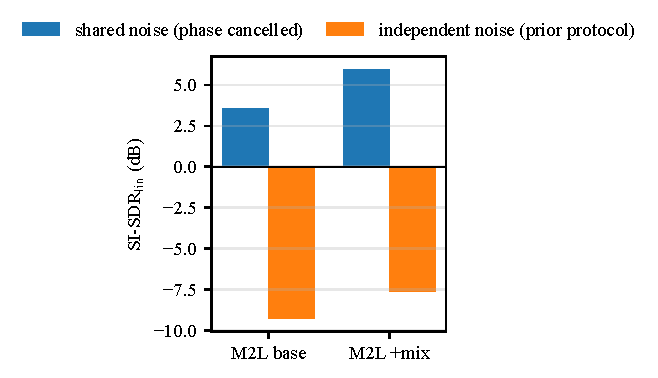
\includegraphics[width=0.82\linewidth]{figures/fig_protocol.pdf}
  \caption{Decode-noise protocol confound (Music2Latent, MUSDB18,
  $\alpha{=}0.5$). The same checkpoints score deeply negative under
  independent-noise decoding and positive under shared-noise decoding; the
  $\approx{-}8$\,dB figure reflects decoder noise, consistent with phase
  variance, not latent linearity.}
  \label{fig:protocol}
\end{figure}

\subsection{Experimental setup}\label{sec:setup}
The primary model is a waveform autoencoder (DAC-style 1-D convolutional
encoder, HiFi-GAN decoder \cite{kong2020hifigan}, combined multi-scale-STFT and
multi-period discriminator) operating at 44.1\,kHz on 1-second mono chunks,
trained on a ${\sim}$950-hour union of FMA-large, MAESTRO, and MUSDB18-HQ
\cite{rafii2017musdb18}.\footnote{Code, training configurations, pretrained
weights, every metric reported here, and audio examples:
\url{https://github.com/nurdauletakhanov/musicgen}} Two compression regimes are used: $7.66\times$
($d{=}128$) and $15.3\times$ ($d{=}64$). Mixing losses are added either as a
25k-step fine-tune over a converged baseline (v2.x) or from scratch over 250k
steps (v3.x). All runs use a single NVIDIA RTX~5090. Unless noted, metrics are
computed over the full multi-source test set; the $\alpha$-sweep
(\secref{sec:alpha}) uses a source-balanced subsample.

\begin{figure}[t]
  \centering
  \resizebox{0.92\linewidth}{!}{%
  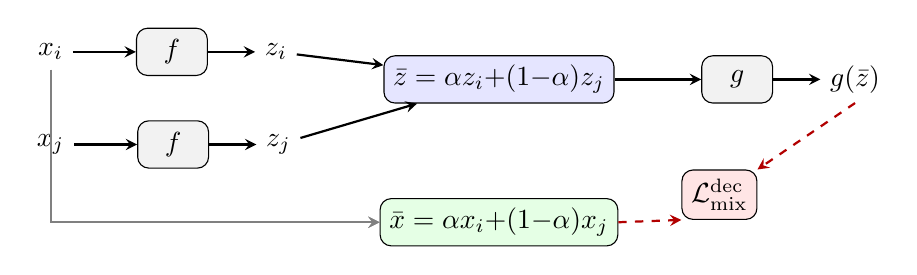
\begin{tikzpicture}[
    node distance=1.0cm and 1.2cm,
    box/.style={draw, rounded corners, minimum height=0.6cm, minimum width=0.9cm, fill=#1},
    box/.default=gray!10, arr/.style={-stealth, thick},
    redarr/.style={-stealth, thick, red!70!black, dashed}]
    \node (x1) {$x_i$};
    \node[below=0.7cm of x1] (x2) {$x_j$};
    \node[box, right=0.8cm of x1] (enc1) {$f$};
    \node[box, right=0.8cm of x2] (enc2) {$f$};
    \node[right=0.6cm of enc1] (z1) {$z_i$};
    \node[right=0.6cm of enc2] (z2) {$z_j$};
    \node[box=blue!10, right=1.1cm of z1, yshift=-0.35cm] (interp) {$\bar{z}=\alpha z_i{+}(1{-}\alpha)z_j$};
    \node[box, right=1.1cm of interp] (dec) {$g$};
    \node[right=0.6cm of dec] (out) {$g(\bar{z})$};
    \node[box=green!10, below=1.2cm of interp] (target) {$\bar{x}=\alpha x_i{+}(1{-}\alpha)x_j$};
    \node[box=red!10, right=0.8cm of target, yshift=0.35cm] (loss) {$\Ldec$};
    \draw[arr] (x1) -- (enc1); \draw[arr] (x2) -- (enc2);
    \draw[arr] (enc1) -- (z1); \draw[arr] (enc2) -- (z2);
    \draw[arr] (z1) -- (interp); \draw[arr] (z2) -- (interp);
    \draw[arr] (interp) -- (dec); \draw[arr] (dec) -- (out);
    \draw[redarr] (out.south) -- (loss.north east);
    \draw[redarr] (target.east) -- (loss.south west);
    \draw[arr, gray] (x1.south) |- (target.west);
    \draw[arr, gray] (x2.south) |- (target.west);
  \end{tikzpicture}}
  \caption{Decode-mixing loss: encode a pair, interpolate latents, decode, and
  compare to the true waveform mix. Gradients (dashed) flow through the decoder
  and back into the encoder via $\bar{z}$.}
  \label{fig:method}
\end{figure}

\section{Results}\label{sec:results}

\subsection{Which signal causes equivariance? An interventional ablation}\label{sec:ablation}
\tabref{tab:ablation} ablates the loss on the $7.66\times$ GAN autoencoder
(25k-step fine-tunes from a shared converged baseline). Each row differs from
its comparator in exactly one factor: $\Ldec$ and $\Lenc$ against the
baseline (the loss), $\Ldec{+}$disc against $\Ldec$ (the adversarial term),
and frozen-encoder $\Ldec$ against $\Ldec$ (the encoder's freedom to adapt);
the design is not a full factorial. Three observations drive the paper.

\begin{table}[t]
  \centering\small
  \setlength{\tabcolsep}{2.2pt}
  % AUTO-GENERATED by make_tables.py � do not edit by hand (regenerate via make_tables.py).
\begin{tabular}{@{}lccccc@{}}
\toprule
Loss & SDR$_\mathrm{rec}$ & SDR$_\mathrm{lin}$ & SDR$_\mathrm{lin}^\mathrm{gt}$ & $\ell_\mathrm{lat}$ & MixRate \\
\midrule
    baseline (no mix) & +11.3 & +12.0 & +8.0 & 0.068 & 1.203 \\
    $\mathcal{L}_\mathrm{dec}$ & +11.4 & +12.1 & +10.2 & 0.052 & 0.972 \\
    $\mathcal{L}_\mathrm{dec}$ + disc-on-mix & +11.4 & +16.0 & +9.9 & 0.050 & 1.052 \\
    $\mathcal{L}_\mathrm{enc}$ ($\gamma{=}5$) & +11.3 & +12.8 & +8.4 & 0.044 & 1.175 \\
    $\mathcal{L}_\mathrm{enc}$ ($\gamma{=}10$) & +11.3 & +13.1 & +8.5 & 0.039 & 1.165 \\
    $\mathcal{L}_\mathrm{enc}$ ($\gamma{=}20$) & +11.3 & +13.5 & +8.7 & 0.034 & 1.153 \\
    $\mathcal{L}_\mathrm{dec}$ frozen-enc & +11.2 & +11.7 & +9.5 & 0.072 & 1.056 \\
\bottomrule
\end{tabular}

  \caption{Mechanism ablation on the GAN autoencoder ($7.66\times$, full test
  set, $\alpha{=}0.5$). SDR$_\mathrm{lin}$ is decode-vs-decode;
  SDR$_\mathrm{lin}^\mathrm{gt}$ is vs.\ ground truth. Single seed.}
  \label{tab:ablation}
\end{table}

\textbf{(1) Reconstruction is unaffected.} SDR$_\mathrm{rec}$ is flat across all
configurations ($11.2$--$11.4$\,dB), and so is FAD ($0.044$--$0.046$): the
mixing loss buys equivariance for free, on both a sample-wise and a
distributional measure of quality.

\textbf{(2) The decode-mixing loss is the active ingredient; the discriminator
on the mixed path is not.} On the ground-truth metric, $\Ldec$ alone improves
SDR$_\mathrm{lin}^\mathrm{gt}$ from $8.0$ to $10.2$\,dB and is the only run with
MixRate $<1$ ($0.97$). Adding an adversarial term to the mixed path
(``+disc-on-mix'') does \emph{not} improve ground-truth equivariance
($9.9$\,dB, MixRate $1.05$), yet it dramatically inflates the decode-vs-decode
SDR$_\mathrm{lin}$ ($12.1\!\to\!16.0$\,dB). The discriminator pulls the two
decode paths onto a common realistic manifold (our hypothesis), raising their mutual SI-SDR
without moving either toward $\bar{x}$. This is direct evidence that
SDR$_\mathrm{lin}$ is gameable, and that given $\Ldec$ no adversarial term is
needed; whether the discriminator has an effect on its own, without $\Ldec$,
is not tested here.

\textbf{(3) The effect is carried through the decoder.} The encoder-only
variant $\Lenc$ drives $\ell_\mathrm{lat}$ lowest but leaves MixRate high
($1.15$--$1.18$): it linearizes the encoder without making the decoder
equivariant. Conversely, training only the decoder under $\Ldec$ with the
encoder frozen retains most of the gain ($9.5$\,dB versus $10.2$ joint and
$8.0$ baseline) while leaving encoder linearity unimproved
($\ell_\mathrm{lat}$ $0.072$). Joint training is best among the tested
configurations.

\subsection{Intervening on compression and architecture}\label{sec:general}
\tabref{tab:crossarch} extends the recipe along two axes. \textbf{Compression:}
trained \emph{from scratch} at $15.3\times$ (v3.1), the mixing model matches its
no-mixing control (v3.0) on reconstruction ($9.9$ vs.\ $10.0$\,dB) while
improving ground-truth equivariance by $+1.7$\,dB
(SDR$_\mathrm{lin}^\mathrm{gt}$ $6.8\!\to\!8.6$), MixRate ($1.19\!\to\!1.05$),
and encoder linearity ($\ell_\mathrm{lat}$ $0.078\!\to\!0.057$). FAD, however, rises from $0.052$ to $0.061$ (\tabref{tab:crossarch});
whether that is perceptible is untested, so ``no quality cost'' is
established at $7.66\times$ (\tabref{tab:ablation}) and only for
SDR$_\mathrm{rec}$ at $15.3\times$. Because v3.0 is
a matched control (same architecture, compression, and schedule, mixing
disabled), this isolates the loss's contribution and shows the effect is not
an artifact of the looser $7.66\times$ rate or of warm-starting.
\textbf{Level preservation.} SI-SDR discards gain, so we also report the gain
it fits (source-balanced subsample): the decoded mix comes out $1.6$\,dB too
quiet for the no-mixing model but $0.9$\,dB for $\Ldec$, the same as each
model's plain-reconstruction level error ($0.8$\,dB); at $15.3\times$,
$1.8$ versus $1.0$\,dB against $0.9$. The loss thus restores level as well as
shape, so Eq.~\ref{eq:equiv} holds beyond scale up to the decoder's own
reconstruction bias. \textbf{Architecture:} we fine-tune the published
Music2Latent \cite{pasini2024music2latent} consistency autoencoder with the
decode-mixing objective, the additivity supervision of
\cite{torres2026linearity} on its own architecture, using its native
consistency loss on the mixed pair in place of the discriminator; this is the
matched comparison in which only the decoder class differs from the GAN
autoencoder. A continued-training control, the same
fine-tune with the mixing terms disabled, moves equivariance by
$<0.2$\,dB and \emph{worsens} FAD, so the mixing model's gain is attributable
to the loss, not to domain adaptation. Both decode-vs-decode and ground-truth
metrics agree on the improvement, confirming it is not a measurement artifact.
Absolute SDR$_\mathrm{lin}^\mathrm{gt}$ remains negative on Music2Latent because
its consistency decoder is phase-incoherent with raw waveforms; the latent
\emph{geometry} improves (MixRate, $\ell_\mathrm{lat}$) but a consistency
decoder does not convert this into clean waveform arithmetic as the GAN decoder
does, so we report the GAN autoencoder as the primary result.

\begin{table}[t]
  \centering\small
  \setlength{\tabcolsep}{2.6pt}
  % AUTO-GENERATED by make_tables.py — do not edit by hand (regenerate via make_tables.py).
\begin{tabular}{@{}lccccc@{}}
\toprule
Model & SDR$_\mathrm{rec}$ & SDR$_\mathrm{lin}$ & SDR$_\mathrm{lin}^\mathrm{gt}$ & MixRate & FAD \\
\midrule
    GAN AE, 7.66$\times$, no mix & +11.3 & +12.0 & +8.0 & 1.203 & 0.045 \\
    GAN AE, 7.66$\times$, +mix & +11.4 & +12.1 & +10.2 & 0.972 & 0.044 \\
    GAN AE, 15.3$\times$, no mix & +10.0 & +10.6 & +6.8 & 1.187 & 0.052 \\
    GAN AE, 15.3$\times$, +mix & +9.9 & +14.6 & +8.6 & 1.046 & 0.061 \\
    M2L, no mix (baseline) & -3.3 & +5.0 & -9.6 & 1.101 & 0.127 \\
    M2L, fine-tune control & -3.1 & +5.1 & -9.5 & 1.125 & -- \\
    M2L, +mix & -2.6 & +6.9 & -7.8 & 1.086 & 0.119 \\
\bottomrule
\end{tabular}

  \caption{Generalization across compression and architecture (full test set,
  $\alpha{=}0.5$, EMA weights for Music2Latent). The M2L ``fine-tune control''
  is the continued-training baseline with mixing disabled.}
  \label{tab:crossarch}
\end{table}

\begin{table}[t]
  \centering\small
  % AUTO-GENERATED by make_tables.py — do not edit by hand (regenerate via make_tables.py).
\begin{tabular}{@{}lcccc@{}}
\toprule
SDR$_\mathrm{lin}^\mathrm{gt}$ & FMA & MAESTRO & MUSDB & all \\
\midrule
    7.66$\times$, no mix & +6.8 & +13.8 & +6.2 & +8.0 \\
    7.66$\times$, +mix & +8.9 & +16.9 & +8.2 & +10.2 \\
    \quad $\Delta$ & \textbf{+2.1} & \textbf{+3.1} & \textbf{+2.0} & \textbf{+2.3} \\
    \midrule
    15.3$\times$, no mix & +5.8 & +12.0 & +5.5 & +6.8 \\
    15.3$\times$, +mix & +7.2 & +15.1 & +6.7 & +8.6 \\
    \quad $\Delta$ & \textbf{+1.4} & \textbf{+3.2} & \textbf{+1.2} & \textbf{+1.7} \\
\bottomrule
\end{tabular}

  \caption{Ground-truth equivariance per test domain (dB). Each $\Delta$ is
  against the matched no-mixing control at the same compression rate. The gain
  is present on every domain, not carried by one.}
  \label{tab:persource}
\end{table}

\textbf{The gain is not domain-driven.} Our test set spans three acoustically
distinct domains: crowd-sourced indie production (FMA), solo piano
(MAESTRO), and multi-track studio mixes (MUSDB18). \tabref{tab:persource}
breaks SDR$_\mathrm{lin}^\mathrm{gt}$ out by domain against the matched
no-mixing control at each compression rate. The improvement appears on all
three at both rates ($+2.0$ to $+3.1$\,dB at $7.66\times$; $+1.2$ to
$+3.2$\,dB at $15.3\times$), so it reflects a property of the learned latent
space rather than an artifact of one recording style. The absolute ordering
(MAESTRO easiest, MUSDB hardest) tracks reconstruction difficulty and is
preserved by the mixing loss.

\subsection{Downstream: latent-arithmetic stem removal}\label{sec:downstream}
We remove a stem by latent subtraction,
$\hat{x}=g(f(x_\mathrm{mix})-f(x_\mathrm{stem}))$, and measure SI-SDR against
the true residual on the MUSDB18 test set. This is an \emph{oracle} setting:
the removed stem is available and encoded, so it tests the representation's
arithmetic, not blind separation; its use is latent-domain editing when stem
codes exist, as in a pipeline that stores compressed stems or a latent
generative model that composes sources without decoding each. Subtraction
uses coefficients $(1,-1)$, which Eq.~\ref{eq:equiv} does not cover
(\secref{sec:intro}), so we report raw subtraction and the origin-corrected
form $g(f(x_\mathrm{mix})-f(x_\mathrm{stem})+f(0))$, exact for affine $f,g$.
We also report the \emph{linearity tax}
$\mathrm{gap}=\mathrm{SISDR}(g(f(x_\mathrm{res})),x_\mathrm{res})-\mathrm{SISDR}(\hat{x},x_\mathrm{res})$,
the shortfall against the model's own encode--decode ceiling.

\begin{table}[t]
  \centering\small
  \setlength{\tabcolsep}{2.2pt}
  % AUTO-GENERATED by make_tables.py — do not edit by hand (regenerate via make_tables.py).
\begin{tabular}{@{}lcccccc@{}}
\toprule
Model & drums & bass & vocals & other & all & gap$\downarrow$ \\
\midrule
    7.66$\times$ no mix & +4.2 & +0.4 & +5.2 & +3.9 & +3.4 & 5.2 \\
    \quad $+f(0)$ & +8.8 & +6.8 & +9.6 & +8.0 & +8.3 & 0.4 \\
    7.66$\times$ $+\mathcal{L}_\mathrm{dec}$ & +5.7 & +4.9 & +7.2 & +5.1 & +5.7 & 3.0 \\
    \quad $+f(0)$ & +8.5 & +6.9 & +9.4 & +8.3 & +8.3 & 0.5 \\
    7.66$\times$ $+\mathcal{L}_\mathrm{dec}$+disc & +6.2 & +5.4 & +7.5 & +5.0 & +6.0 & 2.6 \\
    \quad $+f(0)$ & +8.5 & +7.0 & +9.3 & +8.1 & +8.2 & 0.4 \\
    \midrule
    15.3$\times$ no mix & +1.2 & -1.6 & +3.0 & +2.1 & +1.2 & 6.6 \\
    \quad $+f(0)$ & +7.3 & +5.8 & +8.8 & +7.2 & +7.3 & 0.5 \\
    15.3$\times$ +mix & +5.4 & +4.7 & +6.9 & +3.9 & +5.2 & 2.5 \\
    \quad $+f(0)$ & +7.3 & +6.1 & +8.5 & +7.2 & +7.3 & 0.4 \\
    \midrule
    M2L +mix & -9.9 & -12.3 & -9.9 & -12.7 & -11.2 & 8.4 \\
\bottomrule
\end{tabular}

  \caption{Stem removal via latent subtraction (SI-SDR, dB; MUSDB18 test).
  Higher is better; ``gap'' is the linearity tax against each model's own
  encode--decode ceiling (lower is better). ``$+f(0)$'' rows add the encoded
  silence to the subtracted latent (origin correction).}
  \label{tab:subtraction}
\end{table}

\textbf{Raw subtraction favours the mixing loss; origin correction removes the
difference.} Raw, $\Ldec$ roughly doubles subtraction quality at $7.66\times$
($+3.4\!\to\!+5.7$\,dB) and the matched $15.3\times$ pair goes from $+1.2$ to
$+5.2$\,dB. Adding $f(0)$, one encode of silence, lifts \emph{every} model to
within $0.5$\,dB of its ceiling (\tabref{tab:subtraction}): $+2.0$ to
$+6.0$\,dB per model, on all 49 tracks. With the origin corrected the loss no
longer helps subtraction: $\Ldec$ versus no mixing is $-0.03$\,dB (95\%
track-cluster CI $[-0.15,+0.11]$) and the $15.3\times$ pair $+0.01$\,dB
($[-0.19,+0.21]$). The raw advantage was the no-mixing models' larger latent
offset ($\lVert f(0)\rVert$ $6.6$ versus $5.4$ at $7.66\times$, $18.1$ versus
$14.8$ at $15.3\times$), which coefficient-sum-zero arithmetic pays for. What
the loss buys is convex equivariance (Tables~\ref{tab:ablation}
and~\ref{tab:persource}); subtraction needs the origin, a free post-hoc fix.

\textbf{Baselines without latent arithmetic.} Returning the unchanged mixture
scores $+17.1$\,dB against the residual (the removed stem is a small share of
the energy), above every autoencoder's ceiling, so this metric cannot certify
removal in absolute terms; it measures arithmetic relative to the model's own
reconstruction. Within the model, autoencoding the mixture and doing nothing
scores $+2.2$\,dB ($+1.7$ at $15.3\times$), and decoding mixture and stem
separately and subtracting waveforms scores $+7.5$ ($+6.5$). Raw latent
subtraction is below waveform subtraction for every model (by $1.3$ to
$5.2$\,dB); origin-corrected latent subtraction is above it for every model,
by $+0.7$ to $+0.9$\,dB (track-cluster CIs exclude zero; $80$--$92\%$ of
tracks), with or without the mixing loss.

\textbf{How much of this is measurement noise?} Units from one recording are
correlated, so the resampling unit is the track: a paired cluster bootstrap
draws the 49 tracks with replacement ($10^4$ resamples). Raw contrasts sit far
outside evaluation variance ($\Ldec$: $+2.33$\,dB $[+2.11,+2.54]$;
$15.3\times$: $+4.02$\,dB $[+3.71,+4.34]$; all 49 tracks), and the corrected
contrasts are indistinguishable from zero, as above. Unit-level resampling
gives intervals about three times narrower; we report track-level ones. They
cover evaluation variance at the tested initialization, not variation across
training runs.

\subsection{Equivariance across mixing ratios}\label{sec:alpha}
Sweeping $\alpha$ on a source-balanced subsample (\figref{fig:alpha}), the
mixing loss \emph{flattens} the equivariance curve: the no-mixing baseline sags
most at the hardest balanced mix ($\alpha{=}0.5$) and recovers toward the
extremes, while mixing models stay near-uniform across $\alpha$ (e.g.\
SDR$_\mathrm{lin}^\mathrm{gt}$ swing of $1.2$\,dB for $\Ldec{+}$disc vs.\
$3.2$\,dB for the baseline). Thus the property holds across mixing ratios, not
only at the trained operating point.

\begin{figure}[t]
  \centering
  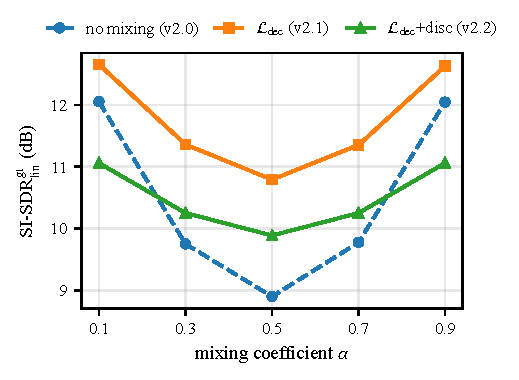
\includegraphics[width=0.82\linewidth]{figures/fig_alpha.pdf}
  \caption{Ground-truth equivariance vs.\ mixing coefficient $\alpha$
  (source-balanced subsample). The no-mixing baseline sags at the hardest
  balanced mix ($\alpha{=}0.5$); the decode-mixing loss flattens and lifts the
  curve across all $\alpha$.}
  \label{fig:alpha}
\end{figure}
We caution that the decode-vs-decode SDR$_\mathrm{lin}$ is U-shaped in $\alpha$
for \emph{all} models (near-identity mixes are trivially easy), which is a
property of that metric, distinct from the phase-variance confound discussed in
\secref{sec:metrics}.

\section{Conclusion}\label{sec:conclusion}
A controlled study identifies an explicit decode-mixing loss as the training
signal responsible for mixing-equivariance in a waveform autoencoder, obtained
at no measured reconstruction cost. The
loss itself, not an adversarial term on the mixed path, is the active
ingredient for convex equivariance, and the effect transfers across
compression rates. Raw stem subtraction is governed by the latent offset, which
one encode of silence removes for every model, with or without the loss. On a
consistency-model autoencoder the loss improves latent geometry under a
continued-training control without yielding usable waveform arithmetic, so
practical claims are confined to the deterministic GAN decoder.
\textbf{Limitations.} Every comparison is matched at a single initialization;
this identifies the effect of each factor at that initialization but not its
variation across training runs. Our confidence intervals cover evaluation
variance (new tracks), so small differences (e.g.\ $\Ldec$ vs.\ $\Ldec{+}$disc, $0.31$\,dB) remain
within plausible seed variance and we report them as ``comparable.'' Experiments are mono;
consistency-decoder latent arithmetic remains phase-limited; and we conduct no
listening test. Stereo, multi-seed estimates, and latent-diffusion composition
are future work.

\bibliographystyle{IEEEtran}
\bibliography{references}

\end{document}
